\chapter[Integrationsprozesse]{Integrationsprozesse}

Anschließend an die Beschreibung einer datengesteuerten Organisation, dessen Aufbau, Prozesse und Rollen werden innerhalb dieses Kapitels die Herausforderungen und Vorgehenswege zur Transformation in eine datengesteuerte Organisation thematisiert.

\section{Herausforderungen}

Bereits durch das sich äußere, sich schnell wechselnde kompetitive Umfeld einer Organisation, verkompliziert sich der Prozess datengesteuert z. B. Strategieentscheidungen in Organisation zu treffen. \footcite[Vgl.][S. 2]{Pratt.2023} 
Hinzu zu der Geschwindigkeit der Geschäftsumgebung, konnte durch eine Gartner Umfrage festgestellt werden, dass 65 \% der Teilnehmenden im Zeitraum der letzten zwei Jahre (2021-2023) einen Zuwachs in der Komplexität der Entscheidungen verzeichneten. \footcite[Vgl.][S. 65]{Pratt.2023}
Damit ist das Ableitungen von Strategieentscheidungen ein besonders herausforderndes Feld aufgrund der hoch diversen Daten und der Vielzahl von Einflussvariablen. \footcite[Vgl.][S. 3]{Pratt.2023}
Dieser äußere Einfluss wirkt sich dadurch ebenfalls erschwerend auf die internen managementbezogenen und kulturellen Herausforderungen aus, welche durch die Transformation zur datengesteuerten Organisation entstehen. \footcite[Vgl.][S. 15]{Dalpiaz.2020}
Bestätigt wird dies von \Citeauthor*{Dalpiaz.2020} durch die Forschungsergebnisse der Auswertung von 15 Interviews aus neun verschiedenen Software Unternehmen.
Aus den Interviews konnten die folgenden in Abbildung 4.1 dargelegte Herausforderungen in der Transformation zu einer datengesteuerten Organisation identifiziert werden. \footcite[][S. 9]{Dalpiaz.2020}

\begin{figure}[htb]
    \centering
    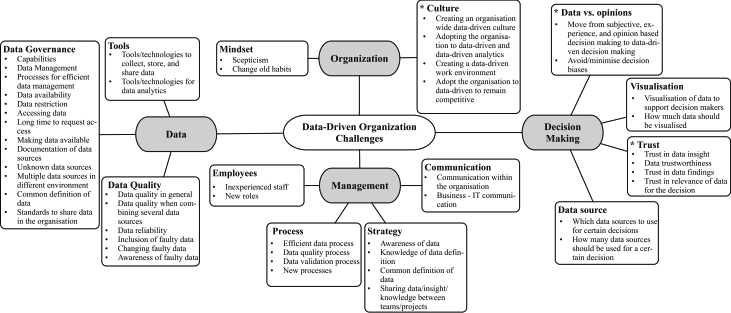
\includegraphics[width=0.95\textwidth]{graphics/DDO challenges.png}
    \caption{Herausforderungen einer datengesteuerten Organisation}
    \label{fig:DDOs challenges}
\end{figure}

Innerhalb der Grafik sind mittels \textbf{*} die drei wichtigsten Herausforderungen faktenbasierte Entscheidungen, Vertrauen und Kultur gekennzeichnet, welche alle 15 Teilnehmenden benannten.
Faktenbasierte Entscheidungen beschreibt die Absicht, subjektive, erfahrungsgestützte und meinungsbasierte Entscheidungen Mittels Daten durchzuführen oder bisherige Prozesse zu unterstützen. \footcite[Vgl.][S. 9]{Dalpiaz.2020}
Ein Einfluss auf die Umsetzung dieser Absicht nimmt die zweite Herausforderung des Vertrauens.
Für faktenbasierte Entscheidungen ist ein hohes Maß an Vertrauen gegenüber vielerlei Aspekte der Daten entlang des Data Science Prozesses notwendig.
Diese Aspekte umfassen die Aufnahme relevanter Daten, die fehlerfreie Aufnahme der Daten, die fehlerlose Verarbeitung der Daten sowie die korrekte Ableitung von für die Entscheidung relevanten Erkenntnissen. \footcite[Vgl.][S. 10]{Dalpiaz.2020}
Die Aufnahme relevanter Daten wird dadurch herausfordernd, dass in etwa 10 \% der Daten insgesamt 90 \% des strategischen Werts enthalten. \footcite[Vgl.][S. 3]{Pratt.2023}
Neben der Geschäftsleitung ist ein solches Vertrauen gegenüber Daten und dessen Auswertung auch als gelebte Kultur der Organisation notwendig. \footcite[Vgl.][S. 4]{Dalpiaz.2020}
Eine gelebte datengesteuerte Kultur kann durch eine geringe Akzeptanz neuer Softwaretools und Arbeitswegen behindert werden. \footcite[Vgl.][S. 15]{Dalpiaz.2020}

Eine notwendige häufig toolgestützte Arbeitsweise ist die unerlässliche Dokumentation der Zusammenarbeit innerhalb des Teams und mit anderen Abteilungen. \footcite[Vgl.][S. 12]{Zhang.2020b}
Innerhalb dieser Dokumentation können z. B. Lösungen für technische Herausforderungen von der Datenbeschaffung bis zum Modelleinsatz festgehalten werden. \footcite[Vgl.][S. 23]{Grossman.2014}
Im Kontext von großen Datenumgebungen müssen technische Herausforderungen gelöst werden, welche zum einen die Aufnahme aller Daten betrifft. \footcite[Vgl.][S. 217]{Elgendy.2014}
Weiterhin muss zum anderen die Flexibilität gewährleistet werden, neue Datenquellen anzubinden und Auswertungen einfach und schnell durchzuführen. \footcite[Vgl.][S. 217]{Elgendy.2014}
Durch Hinzunahme von Technologien wie maschinelles Lernen zur Auswertung von Daten steigen ebenfalls die technischen Herausforderungen.
Maschinelles Lernen bedarf Testsysteme zum Einsatz von Modellen, anpassbare Software zur Überwachung der Modellleistung und Möglichkeiten zur Erläuterung der Modellergebnisse. \footcite[Vgl.][S. 1]{Nahar.2022}

Im gesamten Verlauf der Datenbeschaffung, Modellentwicklung und Ableitung von neuen Optimierungsprozessen sind diverse Teams erforderlich um vorurteilsbehaftete Datenverarbeitung zu vermeiden. \footcite[Vgl.][S. 18]{Zhang.2020b}
Die Beschaffung von Arbeitskräften für ein solches diverses Team stellt eine weitere Herausforderung dar, welche zum einen Bewerber mit datenbezogener Vergangheit aus unteschiedlichen Branchen, oder Universitätsabsolventen und ein ausgearbeitetes Einarbeitungsprogramm bedarf. \footcite[Vgl.][S. 13]{Patil.2011}

Diese Herausforderung allein, sowie in Kombination mit den anderen thematisierten Herausforderungen bedarf einem Rahmenprogramm zur Integration von Data Science in verschiedenste Institutionen. \footcite[Vgl.][S. 1]{Saltz.2017}

\begin{itemize}
    \item outside view (fast and complex decisions)
    \item manageral and cultural challenges
    \item technical challenges
    \item need for DS framework
\end{itemize}

\section{Vorgehensmodelle zur Integration von Data Science}

\begin{itemize}
    \item Conceptual requirements
    \item Design Parameters
    \item Experiment Evolution Model (Microsoft)
    \item CSPG Framework
    \item DI / DS Integration Framework
\end{itemize}